\documentclass[11pt,twoside,twocolumn]{usgsreport}
\usepackage{usgsfonts}
\usepackage{usgsgeo}
\usepackage[figuretoc,tabletoc]{usgsreporta}
\usepackage{lipsum}

\graphicspath{{./Figures/}}

\usepackage{hyperref}
\hypersetup{
    pdftitle={Parallel Krylov Solver for the \textusgs\ Modular Groundwater Flow Model (MODFLOW-2005)},
    pdfauthor={Joseph D. Hughes},
    pdfsubject={Parallel PKS Solver for MODFLOW-2005},
    pdfkeywords={MODFLOW, MPI, Parallel Krylov Solver},
    pdflang={en-US},
    bookmarksnumbered=true,     
    bookmarksopen=true,         
    bookmarksopenlevel=1,       
    colorlinks=true,
    allcolors={blue},          
    pdfstartview=Fit,           
    pdfpagemode=UseOutlines,
    pdfpagelayout=TwoPageRight
}
\urlstyle{rm}

\renewcommand{\cooperator}
{Deltares}
\renewcommand{\reporttitle}
{Parallel Krylov Solver for the \textusgs\ Modular Groundwater Flow Model (MODFLOW-2005)}
\renewcommand{\coverphoto}{Cover.jpg}
\renewcommand{\reportseries}{Techniques and Methods}
\renewcommand{\reportnumber}{6-AXX}
\renewcommand{\reportyear}{2014}

\renewcommand{\theauthors}{Joseph D. Hughes, Jarno Verkaik, and William H. Asquith}
\renewcommand{\thetitlepageauthors}{\theauthors}
\renewcommand{\theauthorslastfirst}{Joseph D. Hughes, Jarno Verkaik, and William H. Asquith}
\renewcommand{\reportcitingtheauthors}{Hughes and others}
\renewcommand{\reportbodypages}{999}

\renewcommand{\reportwebsiteremainder}{tm6AXX}
\ifdef{\usgsissn}{\renewcommand{\usgsissn}{2328-7055}}{}
\renewcommand{\theconventions}{}
\renewcommand{\reportrefname}{References Cited}

\begin{document}
\makefrontcover
\makefrontmatter
\pagestyle{body}

\SECTION{Abstract}
The U.S. Geological Survey \lipsum[2-3]

\SECTION{Introduction}
L-scale ($\lambda_2$) is $\sigma = \sqrt{\pi}\lambda_2$. Recently, Mr. LaTeX has summarized it \citep{ASQUITH20074484}. \lipsum[150-150]

\SECTION{Major Section}
\lipsum[4-5]

\begin{figure}
\begin{center}
	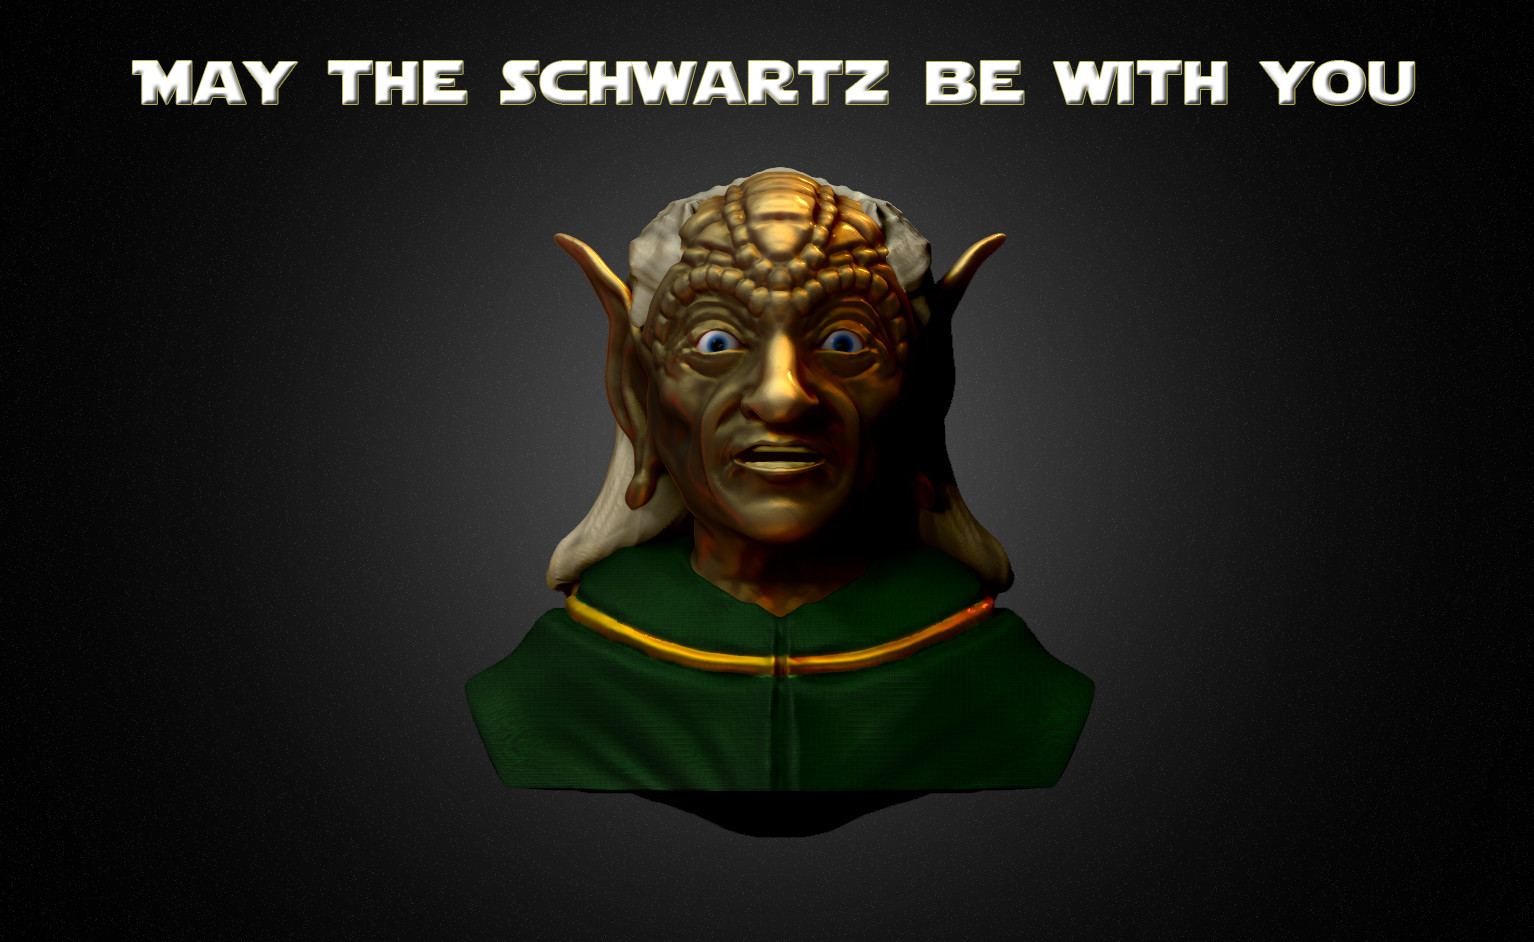
\includegraphics[width=\linewidth]{Cover}

\caption{May the Schwartz be with you.}
\label{fig-1}
\end{center}
\end{figure}


As shown in figure~\ref{fig-1}, \lipsum[34-36]


\subsection{General Discussion}

The number of stations summarized \lipsum[40-50]

\SECTION{Summary}
\lipsum[14-20]

\REFSECTION
\bibliography{USGSLaTeX}
\bibliographystyle{usgs}


\vspace*{\fill}
\clearpage
\pagestyle{backofreport}
\makebackcover
\end{document}